\documentclass[letterpaper,10pt]{extarticle}
\usepackage[utf8]{inputenc}
\usepackage[T1]{fontenc}
\usepackage{graphicx}
\usepackage[x11names]{xcolor}
\usepackage{tikz}
\usepackage[os=win]{menukeys}
\usepackage[americanvoltages,cuteinductors,americanresistors]{circuitikz}
%\ctikzset{bipoles/length=1cm}


%% TODO: Write "final" instead of "draft"
\usepackage[final]{pdfpages}
% \usepackage[draft]{pdfpages}

\usepackage{amsmath,amssymb,textcomp}
\everymath{\displaystyle}

\usepackage{times}
\renewcommand\familydefault{\sfdefault}
\usepackage{tgheros}
%\usepackage[defaultmono,scale=0.85]{droidmono}
\usepackage{droidmono}

\usepackage{enumitem}
%\setlist[enumerate]{itemsep=-1pt}
\usepackage[explicit]{titlesec}

\usepackage{multicol}
\setlength{\columnseprule}{0pt}
\setlength{\columnsep}{15.0pt}

\usepackage{geometry}
\geometry{left=10mm,right=10mm,top=10mm,bottom=15mm}

% custom title
\makeatletter
\renewcommand*{\maketitle}{%
\noindent
\begin{minipage}{0.62\textwidth}

\begin{tikzpicture}
\node[rectangle,rounded corners=6pt,inner sep=6pt,fill=SteelBlue1,text width=.95\textwidth] {\color{black}\huge \@title};
\end{tikzpicture}
\end{minipage}
\hfill
\begin{minipage}{0.37\textwidth}
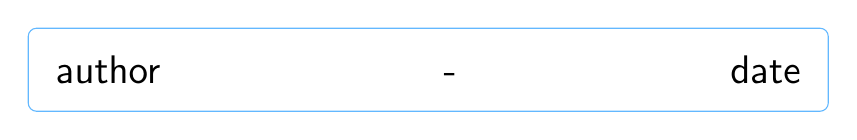
\begin{tikzpicture}
\node[rectangle,rounded corners=3pt,inner sep=10pt,draw=SteelBlue1,text width= 0.78\textwidth] {\Large \@author \hfill-\hfill\@date};
\end{tikzpicture}
\end{minipage}
%\bigskip%\bigskip
}%
\makeatother

% custom section
\newcommand*\sectionlabel{}
\titleformat{\section}
  {\gdef\sectionlabel{}
   \normalfont\sffamily\Large\bfseries\scshape}
  {\gdef\sectionlabel{\thesection\ }}{0pt}
  {
\noindent
\begin{tikzpicture}
\node[rectangle,rounded corners=3pt,inner sep=4pt,fill=DodgerBlue4,text width= 0.95\columnwidth] {\color{white}\sectionlabel#1};
\end{tikzpicture}
  }
\titlespacing*{\section}{0pt}{5pt}{2.5pt}

% custom subsection
\newcommand*\subsectionlabel{}
\titleformat{\subsection}{\normalfont\sffamily\bfseries\scshape}{\subsectionlabel}{0pt}{
\noindent
\begin{tikzpicture}
\node[rectangle,rounded corners=4pt,inner sep=3pt,fill=DodgerBlue3,text width= 0.95\columnwidth] {\color{white}\subsectionlabel#1};
\end{tikzpicture}
}
\titlespacing*{\subsection}{0pt}{5pt}{2.5pt}

% custom subsubsection
\newcommand*\subsubsectionlabel{}
\titleformat{\subsubsection}{\normalfont\sffamily\small\bfseries\scshape}{\subsubsectionlabel}{0pt}{
\noindent
\begin{tikzpicture}
\node[rectangle,rounded corners=3pt,inner sep=3pt,fill=blue!50!yellow,text width= 0.95\columnwidth] {\color{white}\subsubsectionlabel#1};
\end{tikzpicture}
}
\titlespacing*{\subsubsection}{0pt}{5pt}{2.5pt}


\title{MAT265 - Équations différentielles}
\author{Examen Final}
\date{Été 2018}

%\linespread{1.3}

\begin{document}
\maketitle

\begin{multicols*}{2}

%\section{ÉD séparable}
\vspace{-2\baselineskip}
\begin{gather*}
    N(y)\frac{dy}{dx} = M(x) \quad \Rightarrow \quad N(y) \:dy = M(x) \:dx\\
    \int N(y) \:dy = \int M(x) \:dx
\end{gather*}

\section{Équations linéaires d'ordre 1}
%\vspace{-1\baselineskip}
\[y'+P(x)y=Q(x)\]
\centering
\begin{tabular}{rl}
 Étape & Formule\\
 Facteur intégrant & $\mu(x)=e^{\int P(x)dx + C}$ \\
 Solution générale & $y(x)=\frac{\int \mu (x) Q(x) dx +C}{\mu (x)}$
\end{tabular}

\section{É.D. de Bernouilli}
\[y\prime+p(x)y=q(x)y^{n}~~ | n\neq0;1 \]
\centering
\begin{tabular}{rl}
 Étape & Formule\\
 Facteur intégrant & $\mu(x)=e^{\int(1-n)P(x)dx + C}$ \\
 Variable auxiliaire & $y(x)=\frac{\int \mu(x)(1-n) Q(x) dx +C}{\mu (x)}$\\
 Solution générale & $v y^{n-1}=1$
\end{tabular}


\section{É.D. homogène}
\[\frac{dy}{dx}=f\bigg(\frac{y}{x}\bigg)\]
\centering
\begin{tabular}{rl}
 Étape & Formule\\
 Variable auxiliaire & $\int \frac{1}{f(v)-v}dv = \ln|x|+C$\\
 Solution générale & \\
 Si $v$ explicite & $y(x)=xv(x)$\\
 Si $v$ implicite & $v=\frac{y}{x}$
\end{tabular}


\section{É.D. exacte}
\[M(x,y)dx+N(x,y)dy=0\]
\raggedright
Vérification si É.D. est exacte:\\\vspace{5pt}
Si $\frac{\partial M}{\partial y}=\frac{\partial N}{\partial x}$ alors l'É.D. est exacte.
\\\vspace{5pt}
Sinon:\\\vspace{5pt}
Si $\frac{1}{N}\bigg(\frac{\partial M}{\partial y}-\frac{\partial N}{\partial x}\bigg)=f(x)$ alors $\mu(x)=e^{\int f(x)dx}$\\\vspace{5pt}
 Si $\frac{1}{M}\bigg(\frac{\partial N}{\partial x}-\frac{\partial M}{\partial y}\bigg)=g(y)$ alors $\mu(y)=e^{\int g(y)dy}$\\\vspace{5pt}
L'É.D. $\mu M dx+\mu Ndy=0 $ est une É.D. exacte.

% \frac{\partial V}{\partial x}\Leftrightarrow
% $\frac{\partial V}{\partial y}\Leftrightarrow

\[\left \{\begin{matrix} \frac{\partial V}{\partial x}=M\\\\ \frac{\partial V}{\partial y}=N \end{matrix}\right.\Leftrightarrow 
\left \{\begin{matrix} V(x,y)=\int Mdx+C_1(y)\\\\ V(x,y)=\int Ndy+C_2(x) \end{matrix}\right.\]

%\section{Équations linéaires d'ordre 2}
\[Ay''+By'+Cy = f(x) \thickspace|A\neq 0\]

\subsection{Solution générale \hfill}
\[y(x)=y_C+y_P\]

\subsection{Solution complémentaire $y_C$ \hfill}
Équation caractéristique:
\[A\lambda^2+B\lambda+C=0\]
Utiliser cSolve()\\
$1^{er}$ cas:~~$b^2-4ac >0$\\

\centering
$\lambda_1$ et $\lambda_2$ deux racines réelles
\[y(x)=C_1e^{\lambda_1x}+C_2e^{\lambda_2x}\]

\raggedright
$2^{\textrm{ème}}$ cas:~~$b^2-4ac=0$\\

\centering
$\lambda=-b/2a$ racine double
\[y(x)=C_1e^{\lambda x}+C_2xe^{\lambda x}\]

\raggedright
$3^{\textrm{ème}}$ cas:~~$b^2-4ac<0$\\

\centering
$\lambda=\alpha\pm \mathbf{i} \beta$
\[y(x)=C_1e^{\alpha x}\cos(\beta x)+C_2e^{\alpha x}\sin(\beta x)\]
\end{multicols*}

%\break

\subsection{Solution particulière $y_P$}

\begin{tabular}{c|l}
$f(x)$ & Candidat à priori\\\hline
$e^{\alpha x}$ & $Ae^{\alpha x}$\\
$\cos(\omega x)$, $\sin(\omega x)$ & $A\cos(\omega x)+B\sin(\omega x)$\\
$P_{n}(x)=a_n x^n+\dots+a_1 x+a_0\thickspace|a_n\neq0$ & $A_n x^n+A_{n-1} x^{n-1}+\dots+A_1 x+A_0$\\
$e^{\alpha x}\cos(\omega x)$, $e^{\alpha x}\sin(\omega x)$ & $A e^{\alpha x}\cos(\omega x)+B e^{\alpha x}\sin(\omega x)$\\
$P_n (x)e^{\alpha x}$ & $(A_n x^n+A_{n-1} x^{n-1}+\dots+A_1 x+A_0)e^{\alpha x}$\\
$P_n \cos(\omega x)$, $P_n \sin(\omega x)$ & $(A_n x^n+A_1 x+A_0)\cos(\omega x)+(B_n x^n+B_1 x+B_0)\sin(\omega x)$
\end{tabular}

\begin{multicols*}{2}
\raggedright
{\scshape Exception:} Si le candidat à priori fait partie de $y_c$, on le multiplie par la variable indépendante autant de fois que nécessaire.



Résoudre:
\[ A\frac{d^2 y_p}{d^2 x}+B\frac{d y_p}{dx}+C y_p = f(x)\]
On trouve $A$ et $B$ et on remplace dans le candidat $y_p$




\section{Variation des paramètres}
\vspace{-2\baselineskip}
\[ y_p=C_1 (x) y_1 + C_2 (x) y_2\]
\[
W(y_1,y_2) =
\begin{vmatrix}
y_1 & y_2\\
y_1^{\prime} & y_2^{\prime}
\end{vmatrix}
=
(y_1)(y_2^{\prime}) - (y_1^{\prime})(y_2)
\]
Si $W(y_1,y_2) \neq 0$ alors:
\begin{equation*}
    y_p (x)=-y_1(x)\int \frac{y_2(x)r(x)}{W(y_1,y_2)}\:dx+y_2(x)\int\frac{y_1(x)r(x)}{W(y_1,y_2)}\:dx
\end{equation*}



%

\section{Mouvement rectiligne}
\vspace{-2\baselineskip}
\begin{equation*}
m\frac{dv}{dt}=\pm \:mg-kv \;\mid k>0,\;v(0)=\;\textrm{vitesse initiale}
\end{equation*}
\begin{align*}
    a(t) &= \frac{dv}{dt} = \frac{d^2x}{d^2t} = at^2 +a_0\\
    v(t) &= \frac{dx}{dt} = vt+v_0\\
    x(t) &= x_0 + v t + \frac{1}{2}a t^2
\end{align*}

\subsection{Vitesse limite théorique}
\begin{equation*}
v_\infty = \lim_{t\rightarrow 0} v(t)
\end{equation*}

\section{Circuits électriques}
\vspace{-2\baselineskip}
\subsection{Circuit RC}
\[RC\frac{dv_c}{dt}+v_c = v \;\mid v_c(0) = \textrm{tension initial du condensateur}\]

Ensuite, on trouve le courant électrique dans le circuit avec la relation:
\(i(t)=C\frac{dv_c}{dt}\)


\subsection{Circuit RL}
\[L\frac{di}{dt}+Ri=V \;\mid i(0) = \textrm{courant initial souvent}\; i(0)=0\]

\section{Loi de refroidissement Newton}
\vspace{-2\baselineskip} 
\begin{align*}
    \frac{dT}{dt} &= k(T-T_A) \\
    T &= T_A + Ce^{kt}    
\end{align*}
$T$: Température objet, $T_A$: Temp. ambiante, $k$: Constante



\section{Mélanges}
\vspace{-2\baselineskip}
\[ \frac{dq}{dt}=T_e - T_s \;\mid \textrm{où}\; T_e = \textrm{taux à l'entrée et}\; T_s = \textrm{taux à la sortie}\]


%\section{Application des É.D}
\vspace{-2\baselineskip}
\subsection*{Cas particuliers}

\subsubsection{Chute libre}
\raggedright
Équation du mouvement: \(\frac{dv}{dt}+\frac{k}{m}v=g \;\mid v(0)=v_0\)\\
Avec:\\
$k$: coefficient d'amortissement
\begin{gather*}
 v\text{: vitesse} \qquad m\text{: masse} \qquad g\text{: } 9.81 m/s^2
\end{gather*}
É.D linéaire avec:
\begin{gather*}
  p(x)=\frac{k}{m} \qquad  q(x)=g
\end{gather*}
Vitesse limite: \(v_\infty = \frac{mg}{k}\)\\\vspace{2.5pt}
Vitesse instantanée: \[v(t)=v_0 e^{-\frac{k}{m}t}+\frac{mg}{k}(1-e^{-\frac{k}{m}t})\]

\subsubsection*{Circuit RL}
$V_L = L\frac{di}{dt}$\\\vspace{5pt}
$V_R=RI$\\\vspace{5pt}
Loi de kirchoff: \(V_L+V_R=V\)\\
*On suppose V constant\\\vspace{5pt}
Équation: \(\frac{di}{dt}=\frac{R}{L}i=\frac{V}{L} |i(o)=i_0\)\\
É.D de Bernouilli avec:
\begin{gather*}
 y=i \qquad p(x)=\frac{R}{L} \qquad q(x)=\frac{V}{L}
\end{gather*}
Courant limite: \(i_\infty=\frac{V}{R}\)\\
Courant instantané: \(i(t)=i_0e^{-\frac{R}{L}t}+\frac{V}{R}(1-e^{-\frac{R}{L}t})\)\\
$to=\frac{L}{R}=62.2\%$ = constante de temps\\\vspace{5pt}
$T=5e=99.3\%$ = Temps de réponse\\\vspace{5pt}

\subsubsection*{Circuit RC}
$V_R = RI = R_C\frac{dV_C}{dt}$\\\vspace{5pt}
$V_C=\frac{q}{C} = \frac{1}{C}\frac{dq}{dt}$ avec q=charge (coulombs)\\\vspace{5pt}
$i=\frac{dq}{dt}=C\frac{dV_C}{dt}$\\\vspace{5pt}
Loi de Kirchoff: $V=V_R+V_C=R_C\frac{dV_C}{dt}+V_C$\\\vspace{5pt}
Équation caractéristique: \[\frac{dV_C}{dt}+\frac{1}{R_C}V_C=\frac{V}{R_C}\;\mid V_C(0)=V_{C_{0}}\]
*avec V constant\\
\begin{gather*}
    y=V_C \qquad P(x)=\frac{1}{R_C} \qquad q(x)=\frac{V}{R_C}
\end{gather*}
$V_C$ limite: \(V_{C_{\infty}} = V\)\\
$V_C$ instantanée: \(V_C(t)=V_{C_{0}}e^{-\frac{t}{R_C}}+V(1-e^{-\frac{t}{R_C}})\)\\
On suppose que le condensateur n'était pas chargé $V_C(0)=0$\\
Tension instantannée: \(V_C(t)=V(1-e^{-\frac{t}{R_C}})\)\\
$to=RC = 63.21\%$: constante de temps\\
$T=5RC=99.3\%$: temps de réponse

\subsubsection*{Loi de refroidissement de Newton}
$T$ = température de l'objet\\
$M$ = température du milieu\\
$k$ = coefficient de proportionnalité\\
\[\frac{dT}{dt}=-k(T-M) \:\mid  k>0\]
Équation type: \[\frac{dT}{dt}+kT=kM \;\mid T(0)=t_0\]
\begin{gather*}
 y=T \qquad   p(x)=k \qquad q(t)=kM
\end{gather*}
Température limite: $t_\infty=M$\\
Température instantannée: \(T(t)=T_0e^{-kt}+M(1-e^{-kt})\)\\

\subsubsection*{Croissance logistique}
$M$ = population maximale du milieu\\
$P$ = population\\
$v$ = variation de la population\\
Équation type: \(\frac{dv}{dt}+kMv=k \;\mid v(0)=v_0\)
\begin{gather*}
 y=v \qquad    P(x)=km>0 \qquad q(x)=k
\end{gather*}
Variation limite: \(v\infty=\frac{q}{p}=\frac{k}{kM}=\frac{1}{M}\)\\
Variation instantanée: \(P(t)=\frac{P_0 M}{M e^{-kMt}+P_0 (1-e^{- k M t})}\)\\

\subsection*{Méthode générale}
\subsubsection*{Problème type}
\[\frac{dy}{dt}+Py=Q \;\mid y(0)=y_0, \;P \in\; ] 0,\infty[\;,\; Q \in\; ]-\infty,\infty[\]
É.D linéaire et séparable\\
Facteur intégrant: \(\mu(t)=e^{\int P\:dt}\)\\
Condition initiale: \(y(0)=y_0\)\\
\(y_0=\frac{q}{p}+Ce^{-pt}\)\\
\(C=y_0-\frac{q}{p}\)\\
Solution générale: \(y(t)=\frac{\int e^{pt} Q \:dt+C}{e^{pt}}\)\\
\(y(t)=y_0e^{-pt}+\frac{q}{p}e^{-pt}\)\\
Comportement à l'infini: \(y_\infty(t)=\frac{q}{p}\)\\
donc: \(y(t)=y_0e^{-pt}+y_\infty(1-e^{-pt})\)




%\section{Série de Puissances}
\vspace{-1\baselineskip}
\begin{gather*}
p(x)y^{\prime\prime} +q(x)y^{\prime}+r(x)y=0 ~~~  \left\{ \begin{array}{rcl}
y(x_0)& =& y_0\\
y^{\prime}(x_0) & = & y^{\prime}_0
\end{array} \right.
\end{gather*}
\centering
\begin{tabular}{rl}\hline
    $x_0$ & $x_0$ \\
    Points singuliers & \(p(x)=0\) ~~``\(\mathbf{cSolve}()\)'' \\
    Si partie imaginaire & \(R=\sqrt{(x_0)^2 + \beta^2}\)\\
    Sinon & \(R=x_0-\alpha\)\\
    Intervalle de convergence & \(I=]\,x_0-R,\; x_0+R\,[\)\\\hline
\end{tabular}
\\\raggedright
Solution de l'É.D.: ( sauf si $R=0 \Rightarrow I=\emptyset$ )
\vspace{-0.25em}
\begin{equation*}
    \left. y(x)=\sum^{\infty}_{n=0} a_n (x-x_0)^n  \;\;\right| x \in ]\,x_0-R,\; x_0+R\,[
\end{equation*}
\vspace{-0.25em}
\begin{enumerate}[nosep]
    \item Si $x_0 \neq 0$, on pose $v=x\pm x_0$
    \item On remplace $y \longleftarrow \sum{ a_n x^n}$
    \item On obtient:
\end{enumerate}
\centering
\(
    P\sum{ (n-1)n a_n x^{n-2}} +Q\sum{n a_n x^{n-1}}+R\sum{a_n x^n}=0
\)\\\raggedright

\begin{enumerate}[nosep]
\setcounter{enumi}{3}
    \item On remplace $n\leftarrow (n+2), n\leftarrow (n+1)$
    \item On isole le $x^n$ \hspace{1em}[Attention: $x\times x^{n-2}\Rightarrow x^{n-1}$]
    \item On élimine $\Sigma$ et $x^n \;\Rightarrow\;(\Delta_{n+2}\; a_{n+2}+\Delta_{n+1}\; a_{n+1})= 0$
    \item On isole le coefficient d'indice supérieur $a_{n+2}$
\end{enumerate}

\centering
\(
    a_{n+2} = \Delta_{n+1}\; a_{n+1}+\Delta_{n}\; a_{n}
\)
\begin{enumerate}[nosep]
\setcounter{enumi}{7}
    \item On remplace $n\leftarrow (n-2)$
\end{enumerate}
\centering
\(
    a_{n} = \Delta_{n-1}\; a_{n-1}+\Delta_{n-2}\; a_{n-2}
\)

\subsection{Formule de récurrence}
% \vspace{-.75em}
\begin{equation*}
   a_n= \left\{ \begin{array}{ll}
        0 & n<0 \\
        a_0=y(x_0) & n=0\\
        a_1=y^{\prime}(x_0) & n=1\\
        a_n & n\geq 2
    \end{array}\right.
\end{equation*}
% \begin{equation*}
%     y(x)= 
% \end{equation*}
% \vspace{-.75em}

\begin{enumerate}[nosep]
\setcounter{enumi}{8}
    \item On assemble la formule de sommation $y(x)=\Sigma\cdots$
    \item On donne les $n$ premier termes de l'É.D.
\end{enumerate}

\subsubsection{TI}
% \vspace{-.75em}
\begin{equation*}
    a(n):=\left\{ \begin{array}{ll}
        0 & n<0 \\
        a_0=y(x_0) & n=0\\
        a_1=y^{\prime}(x_0) & n=1\\
        \Delta_{n-2}\: a(n-2)+\Delta_{n-1}\; a(n-1) & n\geq 2
    \end{array}\right.
\end{equation*}\\
\vspace{.125em}
{\centering\(\mathbf{seq}(Expr,Var,Inf,Sup)\)}
\vspace{.125em}
% \vspace{-.75em}

\subsection{Calcul des coefficients}
\vspace{-.75\baselineskip}
\begin{align*}
    a_0 &= \frac{2}{P}+\int_{c-\frac{P}{2}}^{c+\frac{P}{2}} y(x) \:dx \\
    a_n &= \frac{2}{P}+\int_{c-\frac{P}{2}}^{c+\frac{P}{2}} y(x)\cos\bigg(n\frac{2\pi}{P}x\bigg) \:dx \\
    b_n &= \frac{2}{P}+\int_{c-\frac{P}{2}}^{c+\frac{P}{2}} y(x)\sin\bigg(n\frac{2\pi}{P}x\bigg) \:dx
\end{align*}
\subsubsection{TI}
\centering
\(
    \mathbf{a0}(c,p,x,fn)\hspace{1em}    \mathbf{an}(c,p,x,fn)\hspace{1em}    \mathbf{bn}(c,p,x,fn) 
\)\\
\raggedright
Représentation graphique
\begin{align*}
    f1(x) &= y(x)\,\mathbf{mod}(x,P)\\
    f2(x)&=y(x)
\end{align*}


\section{Fonction définie par morceaux}
\vspace{-2.5\baselineskip}
\begin{gather*}
f(t) = \left\{ \begin{array}{cc}
 0 & t < \pi \\
 f(t) & t \geq \pi
  \end{array}
  \right.
\;\;\Longleftrightarrow\;\; f(t)u(t-\pi)
\end{gather*}\vspace{-\baselineskip}\\
Inverse (exemple):
\begin{align*}
 y(t)   =&\; (e^{-3t}+e^t)u(t)\tag{1}\\
        &\quad+\frac{1}{4}(e^{t-1}-e^{-3t+3})u(t-1)\tag{2}\\
        &\qquad-\frac{1}{4}(e^{t-2}-e^{-3t+6})u(t-2)\tag{3}
\end{align*}
\begin{equation*}
y(t) = \left\{ \begin{array}{cc}
 0 & t < 0 \\
 (1) & 0\leq t<1\\
 (1)+(2) & 1\leq t<2\\
 (1)+(2)+(3) & t\geq 2
  \end{array}
  \right.
\end{equation*}

\subsubsection{TI}
\centering
\(f(t)\:\mathbf{step}(t-a)\)\\\raggedright
\section{Transformée de Laplace}
%% TODO Ajouter quelque chose p/r au coefficients. As+B
%Linéarité

\subsection{Propriétés}
\noindent
Linéarité \hspace{1em}\(\mathcal{L}\left\{\alpha f(t)+\beta g(t)\right\}= \alpha F(s) + \beta G(s)\)

\subsection{Transformée inverse}

Si $x_0 \neq 0$, on pose \(v=x\pm \Delta x\)\\\raggedright
\begin{enumerate}[nosep]
    \item Mettre en évidence les \(\mathbf{e}^{-at}\)
    \item Modifier l'équation (expand, propFrac)
    \item Résoudre l'équation
\end{enumerate}
Si on veut la réponse sous la forme \(A\sin(\omega t+\phi)\)\\\raggedright

\subsubsection{TI}
\centering
\( \mathbf{expand}() \hspace{1em} \mathbf{propFrac}() \hspace{1em} \mathbf{completeSquare}() \)\\
\(
    \mathbf{tCollect}()\hspace{1em}    \mathbf{tExpand}()\hspace{1em}    \mathbf{ilaplace}() 
\)\\
\raggedright
\section{Série de Puissances}
\vspace{-1\baselineskip}
\begin{gather*}
p(x)y^{\prime\prime} +q(x)y^{\prime}+r(x)y=0 ~~~  \left\{ \begin{array}{rcl}
y(x_0)& =& y_0\\
y^{\prime}(x_0) & = & y^{\prime}_0
\end{array} \right.
\end{gather*}
\centering
\begin{tabular}{rl}\hline
    $x_0$ & $x_0$ \\
    Points singuliers & \(p(x)=0\) ~~``\(\mathbf{cSolve}()\)'' \\
    Si partie imaginaire & \(R=\sqrt{(x_0)^2 + \beta^2}\)\\
    Sinon & \(R=x_0-\alpha\)\\
    Intervalle de convergence & \(I=]\,x_0-R,\; x_0+R\,[\)\\\hline
\end{tabular}
\\\raggedright
Solution de l'É.D.: ( sauf si $R=0 \Rightarrow I=\emptyset$ )
\vspace{-0.25em}
\begin{equation*}
    \left. y(x)=\sum^{\infty}_{n=0} a_n (x-x_0)^n  \;\;\right| x \in ]\,x_0-R,\; x_0+R\,[
\end{equation*}
\vspace{-0.25em}
\begin{enumerate}[nosep]
    \item Si $x_0 \neq 0$, on pose $v=x\pm x_0$
    \item On remplace $y \longleftarrow \sum{ a_n x^n}$
    \item On obtient:
\end{enumerate}
\centering
\(
    P\sum{ (n-1)n a_n x^{n-2}} +Q\sum{n a_n x^{n-1}}+R\sum{a_n x^n}=0
\)\\\raggedright

\begin{enumerate}[nosep]
\setcounter{enumi}{3}
    \item On remplace $n\leftarrow (n+2), n\leftarrow (n+1)$
    \item On isole le $x^n$ \hspace{1em}[Attention: $x\times x^{n-2}\Rightarrow x^{n-1}$]
    \item On élimine $\Sigma$ et $x^n \;\Rightarrow\;(\Delta_{n+2}\; a_{n+2}+\Delta_{n+1}\; a_{n+1})= 0$
    \item On isole le coefficient d'indice supérieur $a_{n+2}$
\end{enumerate}

\centering
\(
    a_{n+2} = \Delta_{n+1}\; a_{n+1}+\Delta_{n}\; a_{n}
\)
\begin{enumerate}[nosep]
\setcounter{enumi}{7}
    \item On remplace $n\leftarrow (n-2)$
\end{enumerate}
\centering
\(
    a_{n} = \Delta_{n-1}\; a_{n-1}+\Delta_{n-2}\; a_{n-2}
\)

\subsection{Formule de récurrence}
% \vspace{-.75em}
\begin{equation*}
   a_n= \left\{ \begin{array}{ll}
        0 & n<0 \\
        a_0=y(x_0) & n=0\\
        a_1=y^{\prime}(x_0) & n=1\\
        a_n & n\geq 2
    \end{array}\right.
\end{equation*}
% \begin{equation*}
%     y(x)= 
% \end{equation*}
% \vspace{-.75em}

\begin{enumerate}[nosep]
\setcounter{enumi}{8}
    \item On assemble la formule de sommation $y(x)=\Sigma\cdots$
    \item On donne les $n$ premier termes de l'É.D.
\end{enumerate}

\subsubsection{TI}
% \vspace{-.75em}
\begin{equation*}
    a(n):=\left\{ \begin{array}{ll}
        0 & n<0 \\
        a_0=y(x_0) & n=0\\
        a_1=y^{\prime}(x_0) & n=1\\
        \Delta_{n-2}\: a(n-2)+\Delta_{n-1}\; a(n-1) & n\geq 2
    \end{array}\right.
\end{equation*}\\
\vspace{.125em}
{\centering\(\mathbf{seq}(Expr,Var,Inf,Sup)\)}
\vspace{.125em}
% \vspace{-.75em}

\subsection{Calcul des coefficients}
\vspace{-.75\baselineskip}
\begin{align*}
    a_0 &= \frac{2}{P}+\int_{c-\frac{P}{2}}^{c+\frac{P}{2}} y(x) \:dx \\
    a_n &= \frac{2}{P}+\int_{c-\frac{P}{2}}^{c+\frac{P}{2}} y(x)\cos\bigg(n\frac{2\pi}{P}x\bigg) \:dx \\
    b_n &= \frac{2}{P}+\int_{c-\frac{P}{2}}^{c+\frac{P}{2}} y(x)\sin\bigg(n\frac{2\pi}{P}x\bigg) \:dx
\end{align*}
\subsubsection{TI}
\centering
\(
    \mathbf{a0}(c,p,x,fn)\hspace{1em}    \mathbf{an}(c,p,x,fn)\hspace{1em}    \mathbf{bn}(c,p,x,fn) 
\)\\
\raggedright
Représentation graphique
\begin{align*}
    f1(x) &= y(x)\,\mathbf{mod}(x,P)\\
    f2(x)&=y(x)
\end{align*}

\section{Séries de Fourier}
\subsection{Calcul des coefficients}

On pose\hspace{1em}\(
  g(x) = \frac{a_0}{2} + \sum_{n=1}^{\infty} a_n \cos(n\,\omega\,x) +b_n \sin(n\, \omega \,x)
\)\\
\raggedright
On calcule les coefficients:
\begin{align*}
  a_0 &= \frac{2}{L} \int^L_0 g(x) \:dx \\
  a_n &= \frac{2}{L} \int^L_0 g(x)\cos(n\,\omega\,x) \:dx \\
  b_n &= \frac{2}{L} \int^L_0 g(x)\sin(n\,\omega\,x) \:dx
\end{align*}
Paramètres
\begin{tabular}{rcl}
$P$ & : & Période de $g(x)$\\
$L$ & = & $P / 2$\\
$\omega$ & = & $2\pi / P \Leftrightarrow 2\pi/2L \Leftrightarrow  \pi/L$ 
\end{tabular}

\subsection{Avec table}

\begin{enumerate}[nosep]
  \item Tracer le graphique de g(x)
  \item Trouver une fonction similaire dans la table
  \item Écrire la valeur des paramètres
  \item Calculer les proportions
\end{enumerate}

Paramètres
\begin{tabular}{rcl}
\(A_g\) & : & Amplitude de \(g(x)\)\\
\(P_g\) & : & Période de \(f(x)\)\\
\(H\) & : & Écart en \(y\)\\
\(c\) & : & Écart en \(x\)\\
\(A_f\) & : & Amplitude de \( f(x) \)\\
\(P_f\) & : & Période de \(f(x)\)
\end{tabular}

\begin{equation*}
  g(x)= H \pm \frac{A_g}{A_f} f\bigg( \frac{P_f}{P_g} (x-c) \bigg)
\end{equation*}

On remplace dans la série \( f(x) \mid x \leftarrow \frac{P_f}{P_g} (x-c) \)

\subsection{Prolongement périodique}
\begin{equation*}
  f(x) = \frac{a_0}{2} + \sum_{n=1}^{\infty} a_n \cos(n \frac{\pi}{L}x) +b_n \sin(n \frac{\pi}{L}x)
\end{equation*}

\begin{tabular}{llll}
    Prolong. ordinaire & \(a_0\) & \(a_n\) & \(b_n\)\\
    Prolong. pair & \(a_0\) & \(a_n\) & \(b_n=0\) \\
    Prolong. impair & \(a_0=0\) & \(a_n=0\) & \(b_n\)
\end{tabular}
\subsubsection{TI}
%\centering
\(\mathbf{prlgp}(type,l,x,fn)\mid\) type: \(o,p,i\) \hfill\(\mathbf{prlgp\_dev}(type,l,x,fn)\)\\
\centering
\(
    \mathbf{a0p}(L,x,fn)\hspace{1em}    \mathbf{anp}(L,x,fn)\hspace{1em}    \mathbf{bnp}(L,x,fn) 
\)\\
%Applications
\section{Application des É.D. d'ordre 2}
\subsubsection{TI}
\centering
\(\mathbf{solver}(\left\{p,q,r\right\}=g(t),t,y,t_0,y_0,y^{\prime}_0)\)\\

\subsection{Type de régime}
\begin{tabular}{ll}
Régime libre & \(g(t)=0\)\\
Régime non amorti & \(g(t)=0\) et \(b=0\)\\
Régime libre sous-amorti & \(g(t)=0\) et \(b<2\sqrt{c} \rightarrow \Delta <0\)\\
Régime libre sur-amorti & \(g(t)=0\) et \(b>2\sqrt{c} \rightarrow \Delta >0\)\\
Régime libre critique & \(g(t)=0\) et \(b=2\sqrt{c} \rightarrow \Delta = 0\)\\
Régime forcé & \(g(t)\neq 0\)
\end{tabular}
\raggedright

\subsection{Mouv. harmonique (Ressorts)}
\vspace{-1\baselineskip}
\begin{gather*}
m y^{\prime\prime} + \beta y^{\prime} + ky = g(t) \;\;\Longleftrightarrow\;\;
y^{\prime\prime} + \frac{\beta}{m} y^{\prime} + \frac{k}{m}y = \frac{g(t)}{m}
\end{gather*}
Paramètres
\begin{tabular}{rll}
  $m$ & masse & [$kg$]\\
  $\beta$ & coefficient d'amortissement & [$N\cdot s/m$]\\
  $k$ & constante de rappel du ressort & [$N/m$]\\
  $g(t)$ & force externe & [$N$]\\
  $y(t)$ & position p/r à équilibre & [$m$]\\
  $v(t)=\frac{dy}{dt}$ & vitesse & [$m/s$]\\
  $a(t)=\frac{dv}{dt}$ & accélération & [$m/s^2$]
\end{tabular}


\subsubsection{TI}
\centering
\(\mathbf{ressort}(m,b,k,f,y_0,v_0)\)\\
\subsection{Circuit RLC}
{\centering
\resizebox{.1\textwidth}{!}{
\begin{circuitikz}
    \draw (0,0)
    to[R, l=$R$] (2,0)
    to[L, l=$L$] (2,-2)
    to[C, l=$C$] (0,-2)
    to[V, l=$V$, invert] (0,0);
\end{circuitikz}
}
}
\\\raggedright
Voltage au capaciteur:
{\centering
%\begin{gather*}
\(
LC V_c^{\prime\prime} + RC V_c^{\prime} + V_c = V(t)\Longleftrightarrow
V_c^{\prime\prime} + \frac{R}{L} V_c^{\prime} + \frac{1}{LC}V_c = \frac{V(t)}{LC}
\)}\\
%\end{gather*}
Courant:
{\centering\(
%\begin{gather*}
L i^{\prime\prime} + R i^{\prime} + \frac{1}{C}i = E(t)\;\;\Longleftrightarrow\;\;
i^{\prime\prime} + \frac{R}{L} i^{\prime} + \frac{1}{LC}i = \frac{E(t)}{L}
% \end{gather*}
\)}\\
Avec:
\begin{tabular}{rlc}
  $R$ & résistance & [$\Omega$] \\
  $L$ & inductance & [$H$]\\
  $C$ & capacité & [$F$]\\
  $E(t)=V(t)$ & source de puissance & [$V$]\\
  $V_c(t)*C = i(t_0)$ & courant à $t_0$ & [$A$]\\
  $V_c(t_0)=i^{\prime}(t_0)$ & voltage au capaciteur à $t_0$ & [$V$]
\end{tabular}


\subsubsection{TI}
\centering
\(\mathbf{circuit}(R,L,C,E,Vc_0,I_0)\)\\


\section{Algorithme de Runge-Kutta}
\raggedright
\subsection{$1^{\mathrm{er}}$ ordre}

\begin{equation*}
    \left\{ \begin{array}{rcl}
        y^{\prime} & = & x^2+y^2 \\
        y(x_0) & = & y_0
    \end{array}\right.
\end{equation*}

\subsubsection{TI}
\menu[,]{Menu,3,8}
\begin{equation*}
    \left\{ \begin{array}{rcl}
        y1^{\prime} & = & x^2+y1^2 \\
        (x_0,y1_0) & = & y_0
    \end{array}\right.
\end{equation*}

Puis: \menu[,]{\ldots,Runge-Kutta, Tol. erreur: 0.0001, Champ: Aucun}

\subsection{$2^{\mathrm{e}}$ ordre}

\begin{equation*}
    \left\{ \begin{array}{rcl}
        (x-5)y^{\prime\prime} +xy^{\prime}+3y & = & 0 \\
        y(x_0) & = & y_0\\
        y^{\prime}(x_0) & = & y^{\prime}_0
    \end{array}\right.
\end{equation*}

%\raggedright

On transforme l'É.D. en É.D. du $1^{\mathrm{er}}$ ordre.\\
On pose: \( y=y_1 \;\mathrm{ et }\; y^{\prime}=y_2 \Longleftrightarrow y^{\prime\prime}=y^{\prime}_2 \)\\
\subsubsection{TI}
\centering
\(\mathbf{de2to1}(Py^{\prime\prime} +Qy^{\prime}+Ry = 0)\)\\\raggedright

\menu[,]{Menu,3,8}
\begin{equation*}
    \left\{ \begin{array}{rcl}
        y1^{\prime} & = & y2 \\
        (x_0,y1_0) & = & y_0\\
        y2^{\prime} & = & y_2^{\prime} \quad\mathrm{(E.D.}\ 1^{er}\ \mathrm{ ordre)}\\
        (x_0, y2_0) & = & y^{\prime}_0
    \end{array}\right.
\end{equation*}

Puis: \menu[,]{\ldots,Runge-Kutta, Tol. erreur: 0.0001, Champ: Aucun}

\subsection{Éditer les valeurs dans le tableau}

\begin{tabular}{cl}
\keys{ctrl+T} & Afficher/Quitter la table des valeurs\\
\keys{menu+2+5} & Paramètres de la table
\end{tabular}
% 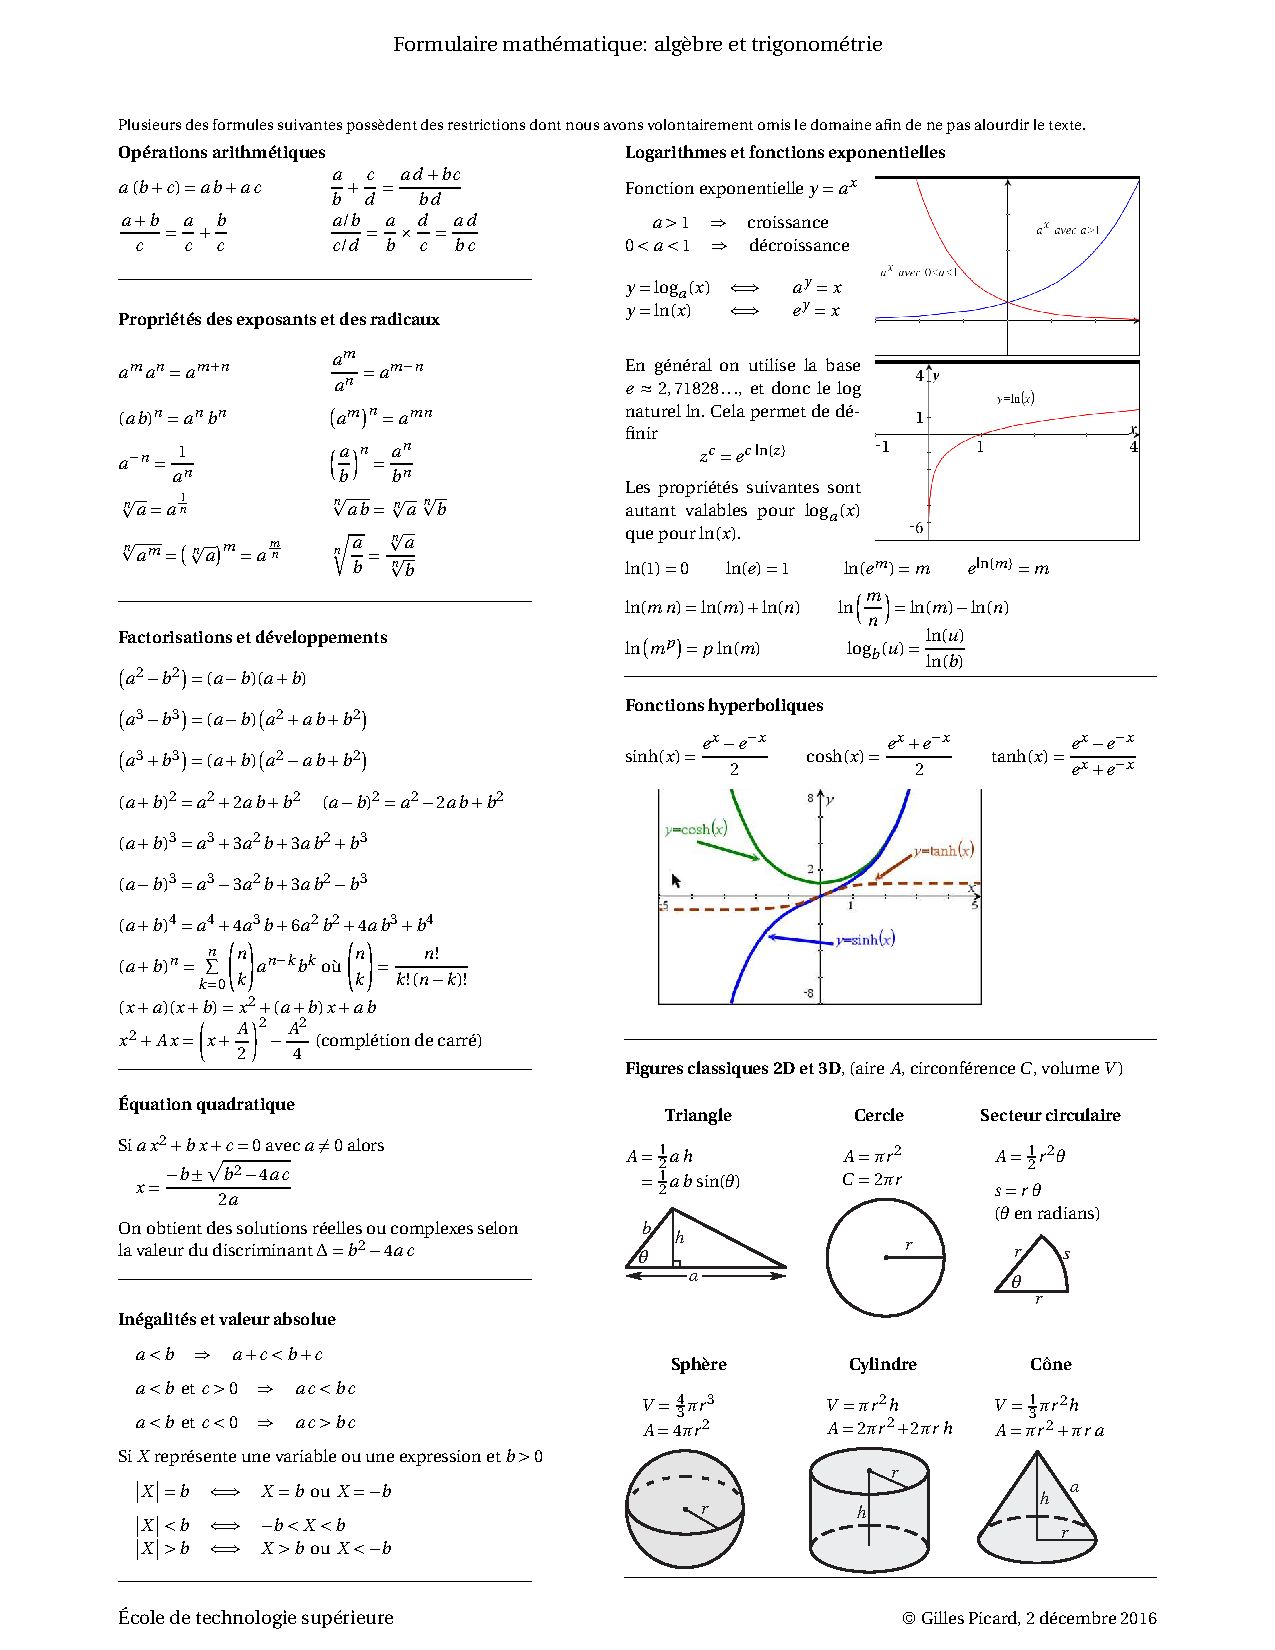
\includepdf[pages=-]{formulaire-algebre-trigo.pdf}
% 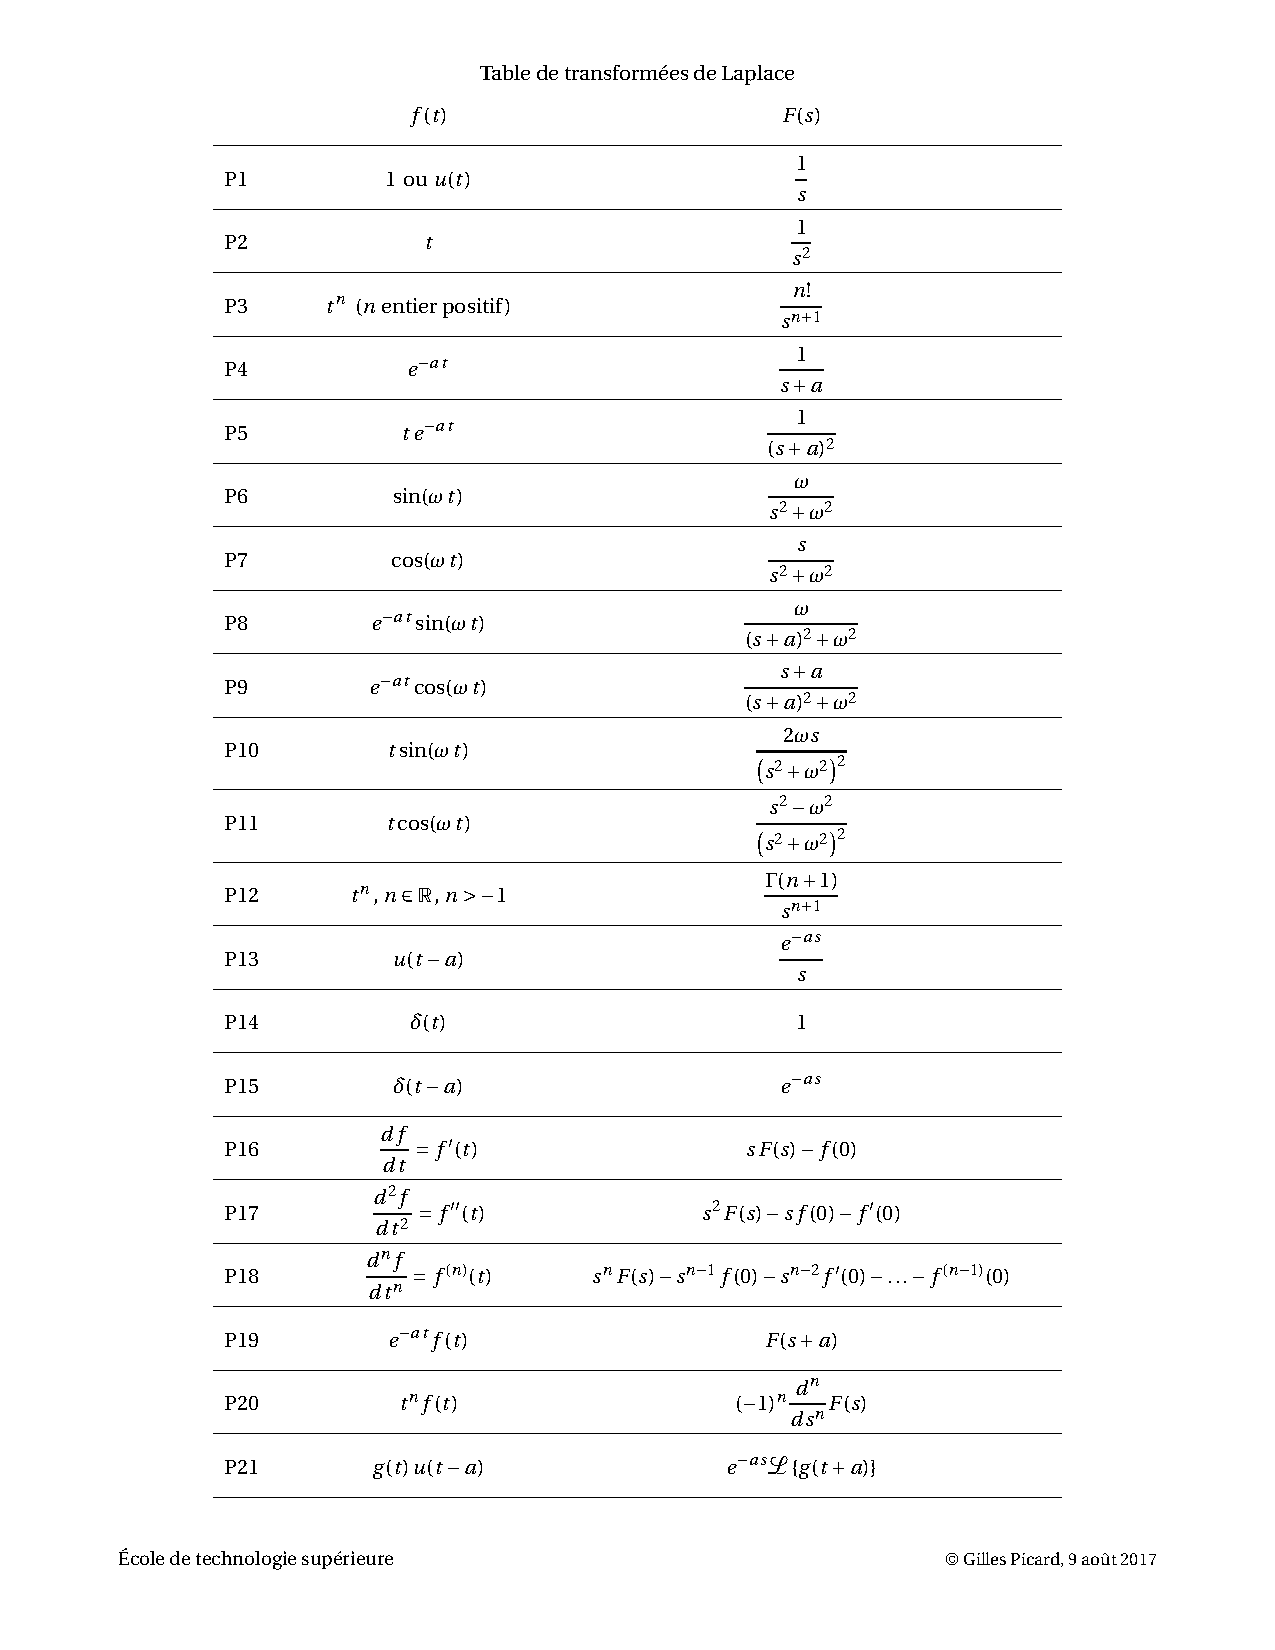
\includepdf[pages=-]{laplace-table.pdf}
% 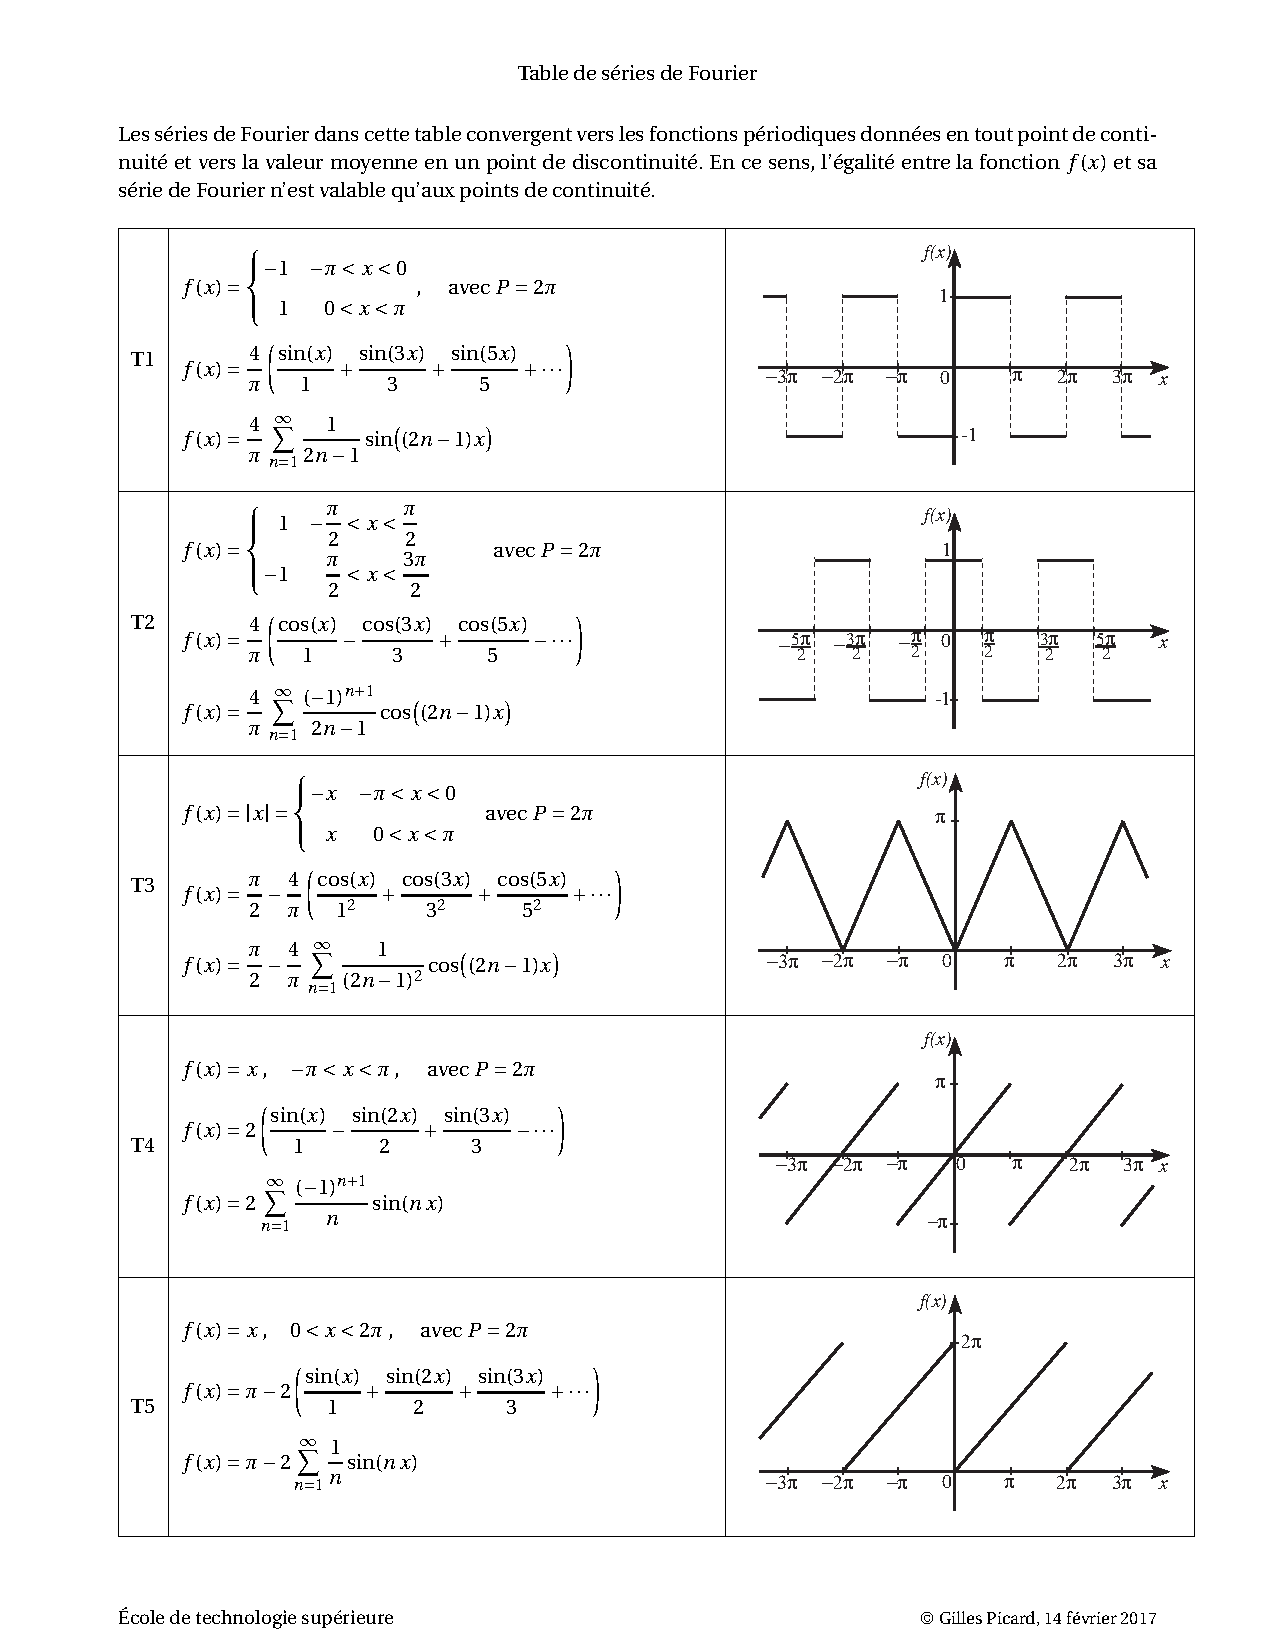
\includepdf[pages=-]{Fourier-table.pdf}
% 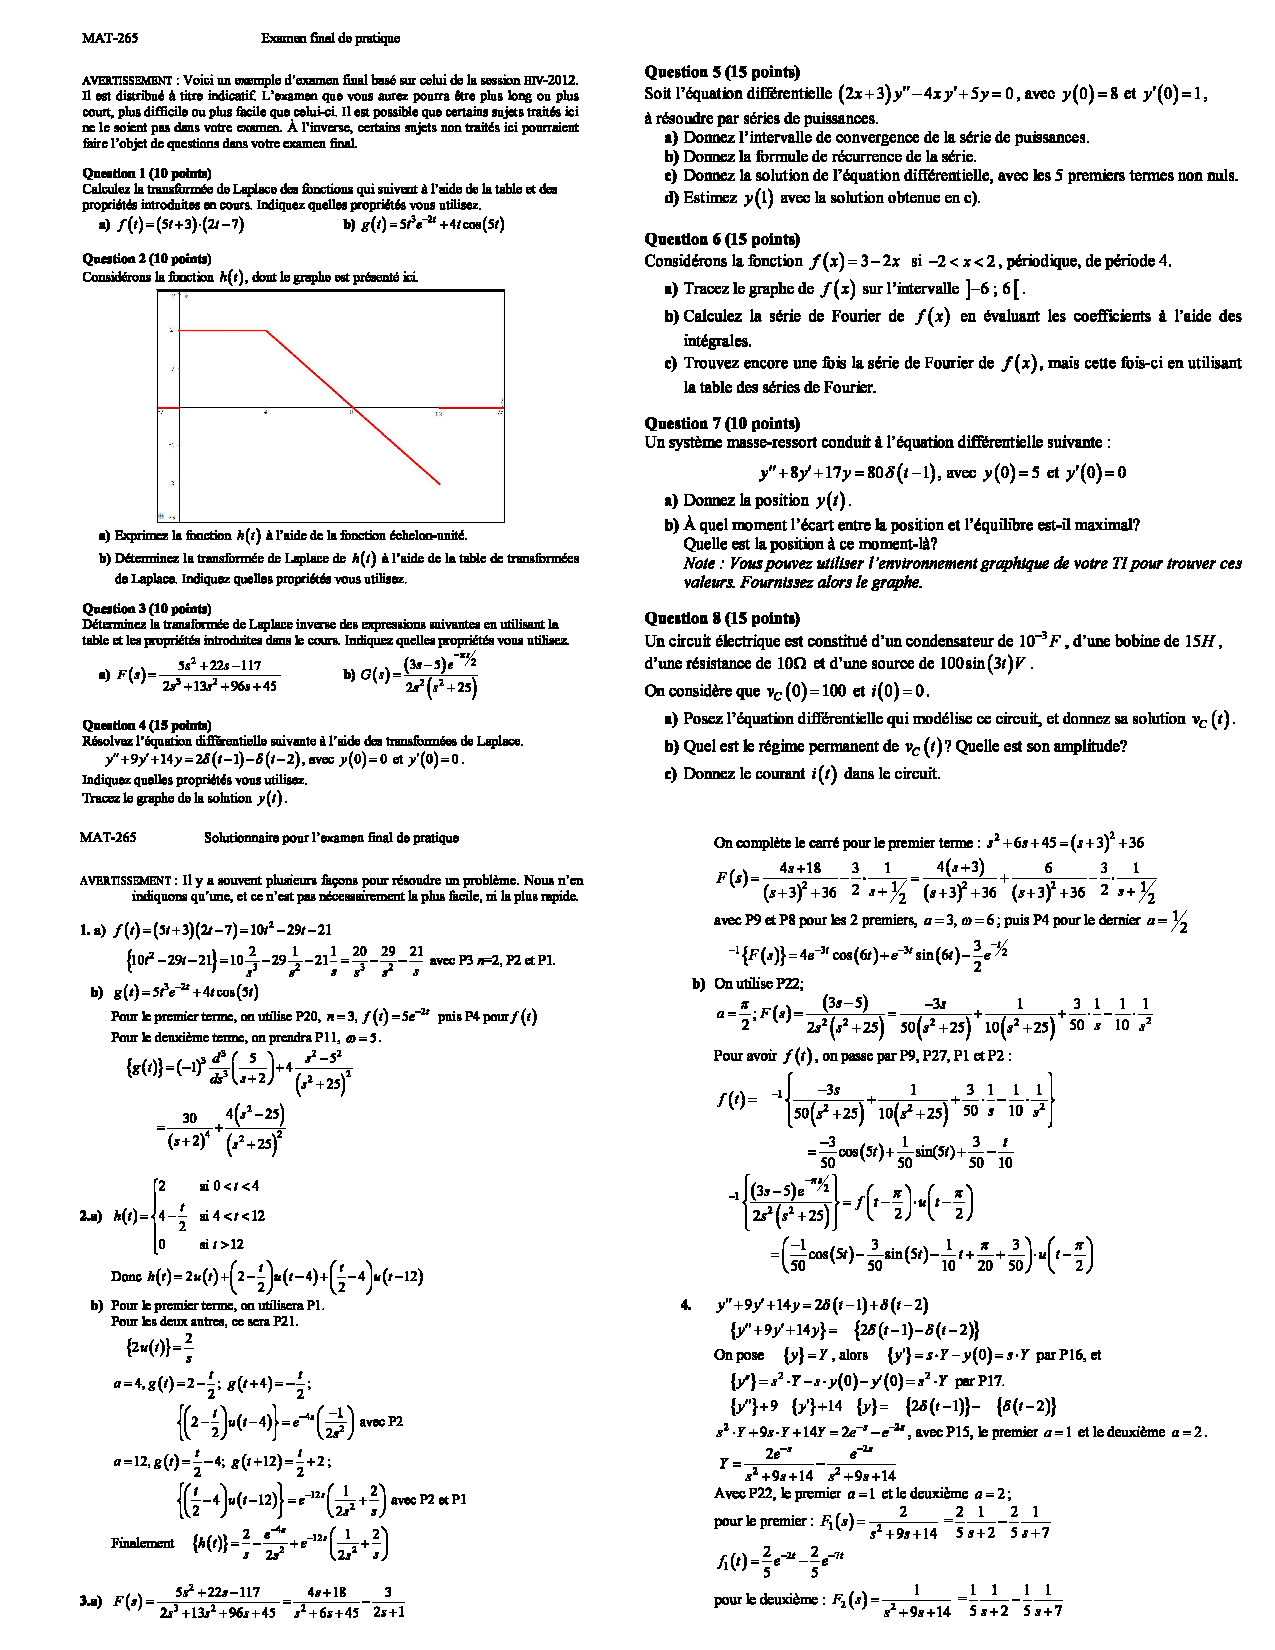
\includepdf[pages=-]{265godsheet.pdf}

\end{multicols*}

\end{document}
